\documentclass[12pt]{beamer}
\usepackage[T2A]{fontenc}
\usepackage[utf8]{inputenc}
\usepackage[english,russian]{babel}
\usepackage{amssymb,amsfonts,amsmath,mathtext, wasysym}
\usepackage{cite,enumerate,float,indentfirst}
\usepackage{makecell}
\usepackage{graphicx}
\graphicspath{{../images/}{images/}{../Thesis/images/}} 
\usepackage{tikz}
\usepackage{calc}
\def\checkmark{\tikz\fill[scale=0.7](0,.35) -- (.25,0) -- (1,.7) -- (.25,.15) -- cycle;}
\def\checkmarksmall{\tikz\fill[scale=0.5](0,.35) -- (.25,0) -- (1,.7) -- (.25,.15) -- cycle;}
\newcommand{\cond}{\;|\;}
\newcolumntype{L}[1]{>{\raggedright\let\newline\\\arraybackslash\hspace{0pt}}m{#1}}
\newcolumntype{C}[1]{>{\centering\let\newline\\\arraybackslash\hspace{0pt}}m{#1}}
\newcolumntype{R}[1]{>{\raggedleft\let\newline\\\arraybackslash\hspace{0pt}}m{#1}}
%\usetheme[secheader]{Boadilla}
%\usecolortheme{seahorse}

\usetheme{Madrid}
\usecolortheme{whale}

\makeatletter
\long\def\beamer@author[#1]#2{%
	\def\insertauthor{\def\inst{\beamer@insttitle}\def\and{\beamer@andtitle}%
		\begin{minipage}{\linewidth}#2\end{minipage}}%
	\def\beamer@shortauthor{#1}%
	\ifbeamer@autopdfinfo%
	\def\beamer@andstripped{}%
	\beamer@stripands#1 \and\relax
	{\let\inst=\@gobble\let\thanks=\@gobble\def\and{, }\hypersetup{pdfauthor={\beamer@andstripped}}}
	\fi%
}
\makeatother
\author[Кочуров М.В.]{%
	\begin{center}
		\large{Кочуров Максим}
	\end{center}
\vspace{2\baselineskip}
	\begin{flushright}
		Научный руководитель:\\
		доцент, к.э.н. Лукаш Е.Н.
	\end{flushright}%
}



\beamertemplatenavigationsymbolsempty

\newcommand{\todo}{\alert}
%%% Основные сведения %%%
\newcommand{\thesisAuthorLastName}{Кочуров}
\newcommand{\thesisAuthorOtherNames}{Максим Вадимович}
\newcommand{\thesisAuthorInitials}{М.В.}
\newcommand{\thesisAuthor}             % Диссертация, ФИО автора
{%
    \texorpdfstring{% \texorpdfstring takes two arguments and uses the first for (La)TeX and the second for pdf
        \thesisAuthorLastName~\thesisAuthorOtherNames% так будет отображаться на титульном листе или в тексте, где будет использоваться переменная
    }{%
        \thesisAuthorLastName, \thesisAuthorOtherNames% эта запись для свойств pdf-файла. В таком виде, если pdf будет обработан программами для сбора библиографических сведений, будет правильно представлена фамилия.
    }
}
\newcommand{\thesisAuthorShort}        % Диссертация, ФИО автора инициалами
{\thesisAuthorInitials~\thesisAuthorLastName}
%\newcommand{\thesisUdk}                % Диссертация, УДК
%{\todo{xxx.xxx}}
\newcommand{\thesisTitle}              % Диссертация, название
{Эконометрическое моделирование динамики корреляций доходностей финансовых стратегий}
\newcommand{\thesisSpecialtyNumber}    % Диссертация, специальность, номер
{38.03.01}
\newcommand{\thesisSpecialtyTitle}     % Диссертация, специальность, название
{Экономика}
\newcommand{\thesisDegree}             % Диссертация, ученая степень
{Бакалавр Экономики}
\newcommand{\thesisDegreeShort}        % Диссертация, ученая степень, краткая запись
{Бакалавр Экономики}
\newcommand{\thesisCity}               % Диссертация, город написания диссертации
{Москва}
\newcommand{\thesisYear}               % Диссертация, год написания диссертации
{2018}
\newcommand{\thesisOrganization}       % Диссертация, организация
{Московский государственный университет имени М.В.Ломоносова}
\newcommand{\thesisOrganizationShort}  % Диссертация, краткое название организации для доклада
{МГУ им. М.В.Ломоносова}

\newcommand{\thesisInOrganization}     % Диссертация, организация в предложном падеже: Работа выполнена в ...
{Московском государственном университете имени М.В.Ломоносова}

\newcommand{\supervisorFio}            % Научный руководитель, ФИО
{Лукаш Евгений Николаевич}
\newcommand{\supervisorRegalia}        % Научный руководитель, регалии
{доцент кандидат экономических наук}
\newcommand{\supervisorFioShort}       % Научный руководитель, ФИО
{Е.Н. Лукаш}
\newcommand{\supervisorRegaliaShort}   % Научный руководитель, регалии
{доцент к.э.н.}


\newcommand{\opponentOneFio}           % Оппонент 1, ФИО
{\todo{Фамилия Имя Отчество}}
\newcommand{\opponentOneRegalia}       % Оппонент 1, регалии
{\todo{доктор физико-математических наук, профессор}}
\newcommand{\opponentOneJobPlace}      % Оппонент 1, место работы
{\todo{Не очень длинное название для места работы}}
\newcommand{\opponentOneJobPost}       % Оппонент 1, должность
{\todo{старший научный сотрудник}}

\newcommand{\opponentTwoFio}           % Оппонент 2, ФИО
{\todo{Фамилия Имя Отчество}}
\newcommand{\opponentTwoRegalia}       % Оппонент 2, регалии
{\todo{кандидат физико-математических наук}}
\newcommand{\opponentTwoJobPlace}      % Оппонент 2, место работы
{\todo{Основное место работы c длинным длинным длинным длинным названием}}
\newcommand{\opponentTwoJobPost}       % Оппонент 2, должность
{\todo{старший научный сотрудник}}

\newcommand{\leadingOrganizationTitle} % Ведущая организация, дополнительные строки
{\todo{Федеральное государственное бюджетное образовательное учреждение высшего профессионального образования с~длинным длинным длинным длинным названием}}

\newcommand{\defenseDate}              % Защита, дата
{23 мая 2018~г.}
\newcommand{\defenseCouncilNumber}     % Защита, номер диссертационного совета
{\todo{Д\,123.456.78}}
\newcommand{\defenseCouncilTitle}      % Защита, учреждение диссертационного совета
{\todo{Название учреждения}}
\newcommand{\defenseCouncilAddress}    % Защита, адрес учреждение диссертационного совета
{\todo{Адрес}}
\newcommand{\defenseCouncilPhone}      % Телефон для справок
{\todo{+7~(0000)~00-00-00}}

\newcommand{\defenseSecretaryFio}      % Секретарь диссертационного совета, ФИО
{\todo{Фамилия Имя Отчество}}
\newcommand{\defenseSecretaryRegalia}  % Секретарь диссертационного совета, регалии
{\todo{д-р~физ.-мат. наук}}            % Для сокращений есть ГОСТы, например: ГОСТ Р 7.0.12-2011 + http://base.garant.ru/179724/#block_30000

\newcommand{\synopsisLibrary}          % Автореферат, название библиотеки
{\todo{Название библиотеки}}
\newcommand{\synopsisDate}             % Автореферат, дата рассылки
{\todo{DD mmmmmmmm YYYY года}}

% To avoid conflict with beamer class use \providecommand
\providecommand{\keywords}%            % Ключевые слова для метаданных PDF диссертации и автореферата
{}
      % Основные сведения

\newcommand{\itemi}{\item[\checkmark]}

\title[Моделирование динамики]{\thesisTitle}
\institute[МГУ]{\vspace{-\baselineskip}\normalsize\thesisOrganizationShort}
\date{\thesisCity, \thesisYear}

\begin{document}
\maketitle
\begin{frame}{Актуальность}
\textbf{Актуальность:}
\begin{itemize}
	\item Торговые алгоритмы -- альтернатива активам
	\item Портфель из торговых стратегий -- возможность лучшей диверсификации
	\item Существует интерес в индустрии к поставлению портфеля из ТС
	\item Отсутствуют исследования на эту тему
\end{itemize}
Исследование актуально и востребовано
\end{frame}
\begin{frame}{Цель}

\textbf{Проблемы:}
\begin{itemize}
	\item Алгоритмы $\ne$ Активы
	\item Алгоритмов много (>700000), нужен отбор
	\item Стратегии составляют люди \\$\rightarrow$ <<проблема оракула>>
	\item[$\blacktriangleright$] Много априорных знаний о распределении доходностях торговых стратегий
\end{itemize}
\vspace{\baselineskip}

\textbf{Цель:} учесть априорные знания о доходностях алгоритмов при формировании портфеля торговых стратегий
\end{frame}
\begin{frame}{Цели и Задачи}
\textbf{Задачи:}
\begin{itemize}
	\item Предложить модель динамики доходности ТС и способ ее оценки
	\item Предложить метод составления портфеля
	\item Оценить модель на реальных данных
	\item Выяснить практическую значимость разработанного метода составления портфеля
\end{itemize}
\end{frame}
\begin{frame}{Преимущества байесовского подхода}
\begin{minipage}{0.6\linewidth}
	\begin{itemize}
		\item Учет экспертных знаний
		\item Интерпретируемость
		\item Гибкость моделирования
		\item Учет неуверенности в значениях параметров
	\end{itemize}
\end{minipage}
\begin{minipage}{0.38\linewidth}
	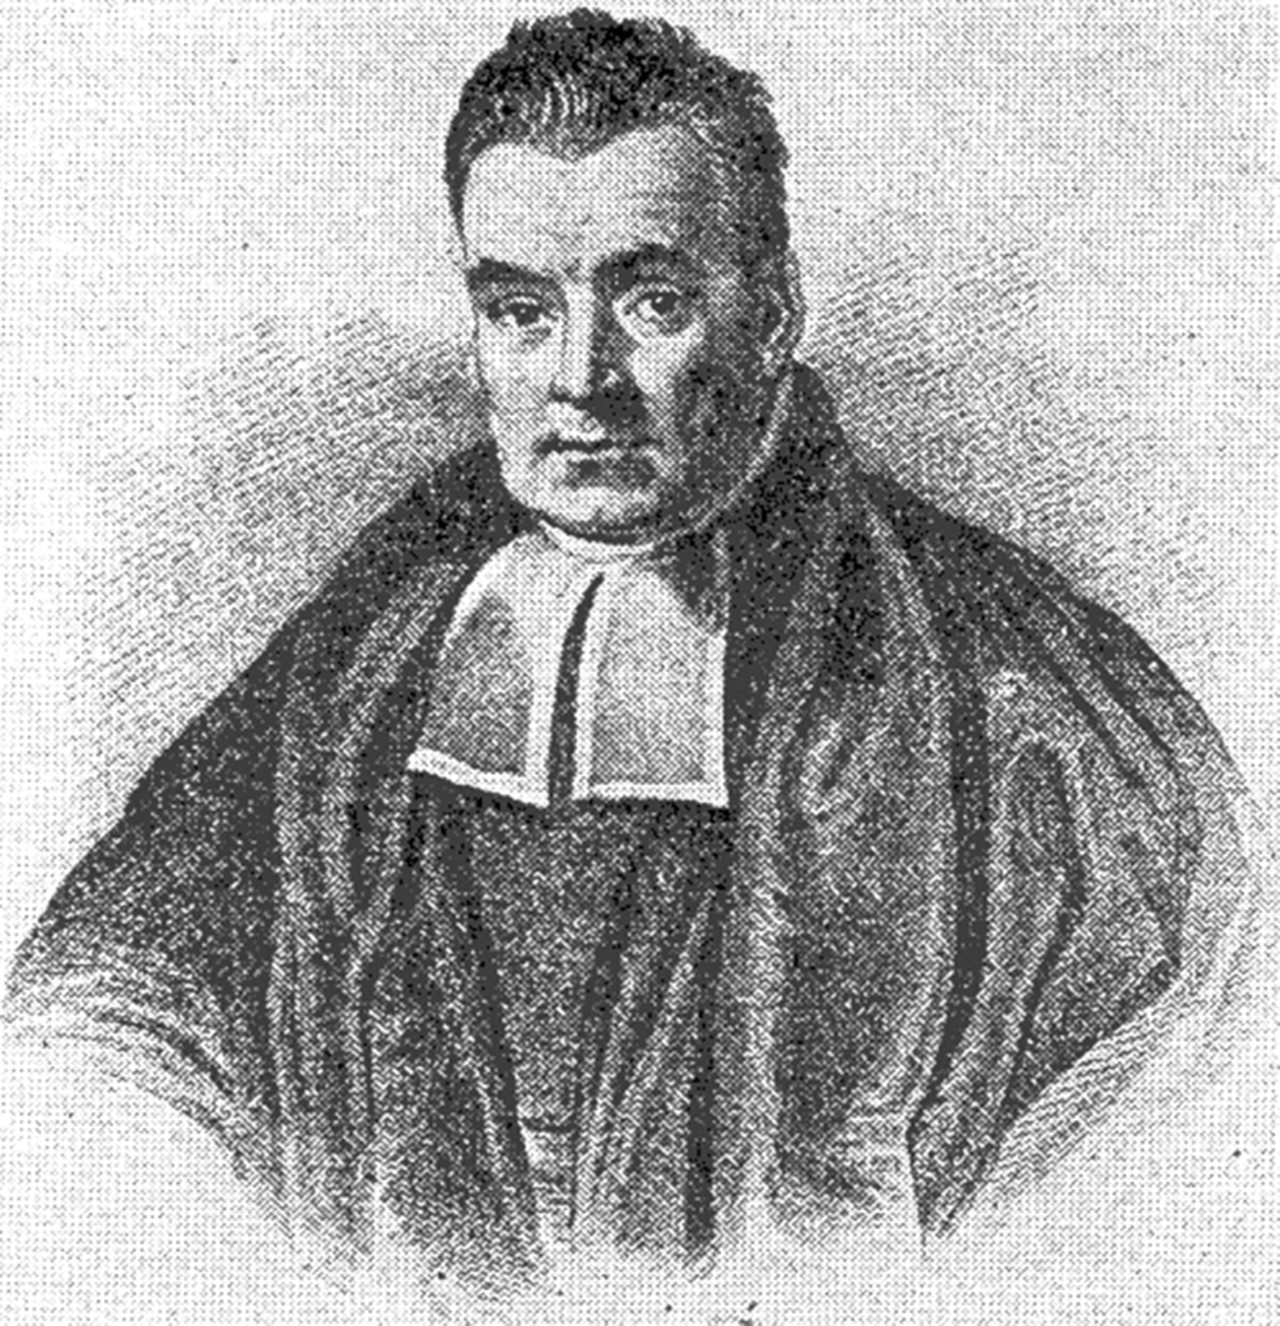
\includegraphics[width=\linewidth]{bayes}
\end{minipage}
\end{frame}
\begin{frame}{Учёт предпосылок}
\begin{itemize}
	\item Точка перелома распределения доходностей
	\begin{itemize}
		\item[>] Структурный сдвиг -- часть модели
	\end{itemize}
	\item<2-> Доходности имеют непостоянную волатильность (Dumas et al., 1998)
	\begin{itemize}
		\item[>] Модели волатильности: GARCH, \textcolor<3->{green}{GPVol}
	\end{itemize}
	\item<4-> Динамика корреляций (Vaga, 1990)
	\begin{itemize}
		\item[>] Модели динамической корреляции: DCC, \textcolor<5->{green}{DECO}
		\item<5->[>] Используем модификацию DECO
		\item<6-|alert@6>[>]Верно ли для доходностей стратегий?
	\end{itemize}
\end{itemize}
\begin{overlayarea}{\textwidth}{5cm} %\myheight is the quantity to be determined
\small
\begin{block}<2->{Преимущества и недостатки}
	\only<2-3>{
		\begin{tabular}{L{.5\linewidth}|L{.5\linewidth}}
			\textbf{GARCH} & \textbf{GPVol}\\
			($-$) сложность с байесовским подходом & ($+$) богаче GARCH\\
			& ($+$) проста в использовании
		\end{tabular}
	}
	\only<4->{
		\begin{tabular}{L{.5\linewidth}|L{.5\linewidth}}
			\textbf{DCC} & \textbf{DECO}\\
			($+$) полная динамика & ($-$) неполная динамика\\
			($-$) не масштабируется & ($+$) масштабируема\\
			 & ($-$) требуется модификация
		\end{tabular}
	}
\end{block}	
\end{overlayarea}

\end{frame}
\begin{frame}{Спецификация модели}
\textbf{Ключевые компоненты:}
\begin{itemize}
	\item Доходности $r_t$ $\sim$ Гауссовский Процесс + шум
	\begin{itemize}
		\item[\checkmarksmall] среднее ГП -- средняя доходность
		
		(о ней много знаем)
	\end{itemize}
	\item<2-> Волатильность $\sigma_t$ $\sim$ Гауссовский Процесс
	\begin{enumerate}
		\item[\checkmarksmall] Идеи GPVol
	\end{enumerate}
	\item<3-> Корреляции доходностей ТС?
	\begin{enumerate}
		\item Динамические $\rightarrow$ модификация DECO с ГП
		\item Статические 
		\item Без корреляций
	\end{enumerate}
	\item<4-> Структурный сдвиг
	\begin{itemize}
		\item[\checkmarksmall] только для средних доходностей
	\end{itemize}
\end{itemize}
\begin{overlayarea}{\textwidth}{5cm}
\only<1>{
	\smiley\ Гауссовский процесс имеет интерпретируемые параметры, позволяет учесть априорные знания
}
\only<2>{
	\smiley\ Учитываем непостоянную волатильность гауссовским процессом
}
\only<3>{
	Для корреляций доходностей несколько вариантов модели, нет работ анализирующих их динамику
}
\end{overlayarea}
\end{frame}
\begin{frame}{Оптимизация портфеля}
\textbf{Метод Монте Карло}

\begin{minipage}{0.49\linewidth}
	\begin{enumerate}
		\item Оцениваем модель
		\item Делаем симуляции доходностей
		\item Оптимизируем матожидание функции полезности инвестора
	\end{enumerate}
\end{minipage}
\begin{minipage}{0.49\linewidth}
	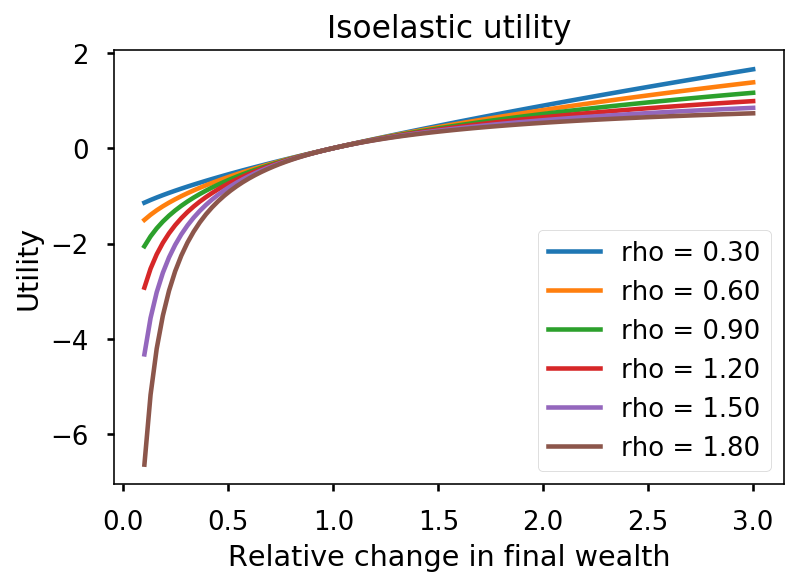
\includegraphics[width=\linewidth]{isoelastic}
	
	Полезность инвестора
\end{minipage}
\end{frame}
\begin{frame}{Оценка байесовской модели}
\textbf{Hamiltonian Monte Carlo}
\begin{tabular}{lr}
\includegraphics[height=2.5em]{pymc3}
&\makecell{\vspace{1.5em}
$\small p(\Theta\cond\mathcal{D}) =
\frac
{p(\mathcal{D}\cond\Theta)p(\Theta)}
{\color{red}{p(\mathcal{D})}}$}
\end{tabular}

\begin{minipage}{.5\linewidth}
	\begin{itemize}
		\item[+] Сэмплирование из сложных распределений
		\item[+] Хорошие условия сходимости
		\item[\checkmarksmall] Требуется непрерывность параметров
	\end{itemize}
\end{minipage}
\begin{minipage}{.48\linewidth}
	\includegraphics[width=\linewidth]{sampleHMC}
\end{minipage}
\end{frame}

\begin{frame}{Данные}
Данные были предоставлены компанией \textbf{Quantopian}
\begin{itemize}
	\item Всего 700000+ алгоритмов за период 4 года
	\item Существует внутренняя система отбора стабильных алгоритмов
	\item Наблюдается эффект стохастической волатильности
	\item Корреляции довольно стабильны во времени
\end{itemize}
Подходят только спецификации со статическими корреляциями
\end{frame}

\begin{frame}{Сравнительный анализ}
\textbf{Бутстрап распределение коэфф. Шарпа (отложенный период)}
\includegraphics[width=\linewidth]{performance-rus}
\end{frame}
\begin{frame}{Заключение}
\begin{itemize}
	\item Предложен метод составления портфеля биржевых торговых
стратегий, учитывающий априорные знания о распределении их доходностей
	\item Эффективность метода по сравнению с бенчмарком подтверждена экспериментально
	\item Предложена модификация базового компонента модели, динамики а именно расширение DECO с использованем гаусовского процессса
\end{itemize}
\end{frame}
\end{document}
